% Slide 36: Tasks and Applications
\begin{frame}{وظایف و کاربردهای داده‌کاوی}
\begin{columns}[T,onlytextwidth]
\begin{column}{0.65\textwidth}
\begin{itemize}
  \item \textbf{وظایف توصیفی} (\lr{Descriptive Tasks})
  \begin{itemize}
    \item کشف الگوها و ساختارهای پنهان در بطن داده‌ها
    \item \textbf{مثال:} کدام کالاها معمولاً همراه با یکدیگر خریداری می‌شوند؟
  \end{itemize}
  \vspace{0.25cm}
  \item \textbf{وظایف پیش‌بینانه} (\lr{Predictive Tasks})
  \begin{itemize}
    \item تخمین مقادیر نامعلوم یک متغیر هدف بر اساس مشاهدات گذشته
    \item \textbf{مثال:} آیا کاربر روی تبلیغ آنلاین کلیک خواهد کرد؟
  \end{itemize}
  \vspace{0.25cm}
  \item \textbf{اصطلاحات متناظر در یادگیری ماشین:}
  \begin{itemize}
    \item توصیفی $\equiv$ \lr{Unsupervised Learning} (یادگیری بدون نظارت)
    \item پیش‌بینانه $\equiv$ \lr{Supervised Learning} (یادگیری بانظارت)
  \end{itemize}
\end{itemize}
\end{column}
\begin{column}{0.32\textwidth}
\begin{center}
  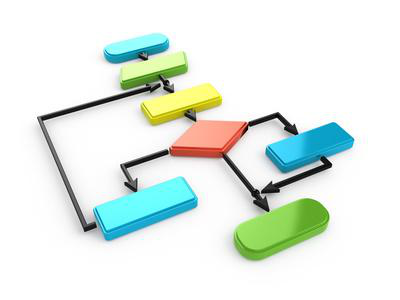
\includegraphics[width=\textwidth,height=3.8cm,keepaspectratio]{images/img_p36_1_188.jpeg}
\end{center}
\end{column}
\end{columns}
\end{frame}

% Slide 37: Data Mining Tasks Overview
\begin{frame}{چهار دسته اصلی وظایف داده‌کاوی}
\begin{columns}[c,onlytextwidth]
\begin{column}{0.62\textwidth}
\begin{itemize}
  \item \textbf{دسته‌بندی} (\lr{Classification}) \quad {\small\color{structure}\textbf{\lr{[Predictive]}}}
  \begin{itemize}
    \item پیش‌بینی برچسب‌های کیفی یا رده‌ها (وظیفه پیش‌بینانه)
  \end{itemize}
  \vspace{0.15cm}
  \item \textbf{رگرسیون} (\lr{Regression}) \quad {\small\color{structure}\textbf{\lr{[Predictive]}}}
  \begin{itemize}
    \item تخمین مقادیر کمی و عددی پیوسته (وظیفه پیش‌بینانه)
  \end{itemize}
  \vspace{0.15cm}
  \item \textbf{تحلیل خوشه‌بندی} (\lr{Cluster Analysis}) \quad {\small\color{teal}\textbf{\lr{[Descriptive]}}}
  \begin{itemize}
    \item گروه‌بندی داده‌های مشابه بدون برچسب (وظیفه توصیفی)
  \end{itemize}
  \vspace{0.15cm}
  \item \textbf{تحلیل وابستگی} (\lr{Association Analysis}) \quad {\small\color{teal}\textbf{\lr{[Descriptive]}}}
  \begin{itemize}
    \item کشف قوانین هم‌آیی میان اقلام سبد خرید (وظیفه توصیفی)
  \end{itemize}
\end{itemize}
\end{column}
\begin{column}{0.35\textwidth}
\begin{center}
  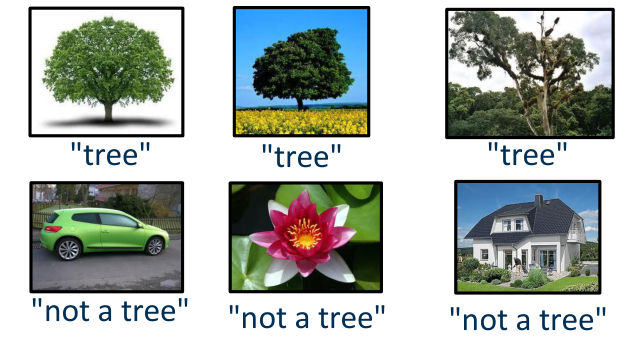
\includegraphics[height=1.1cm,keepaspectratio]{images/thumb_trees_classification.png}\\[0.15cm]
  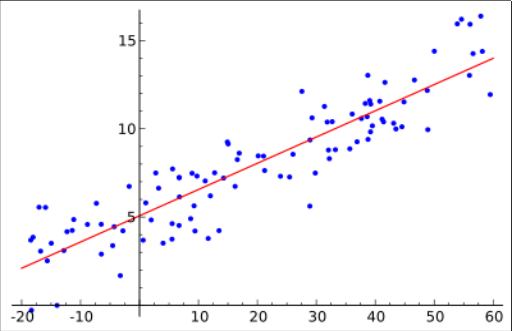
\includegraphics[height=1.0cm,keepaspectratio]{images/img_p37_8_198.png}\\[0.15cm]
  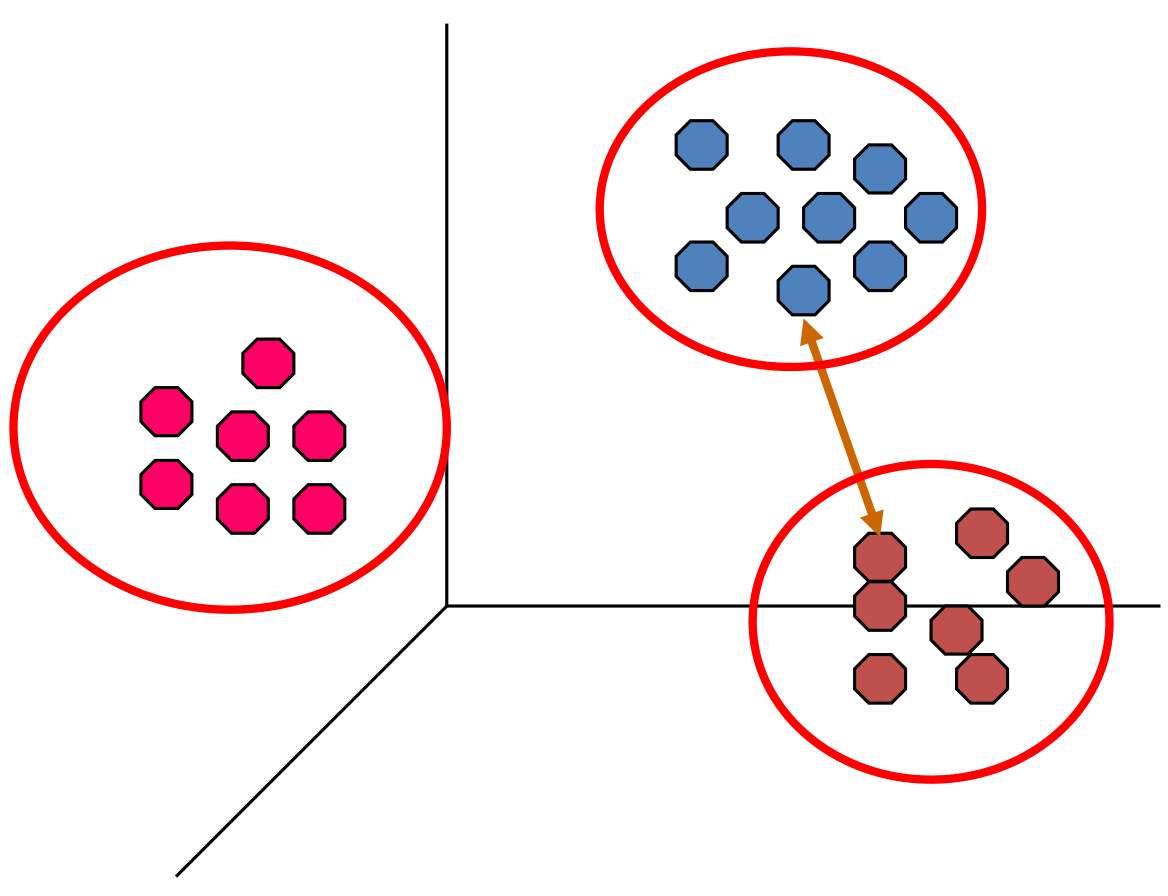
\includegraphics[height=1.2cm,keepaspectratio]{images/diagram_p43_cluster_drawing.png}\\[0.15cm]
  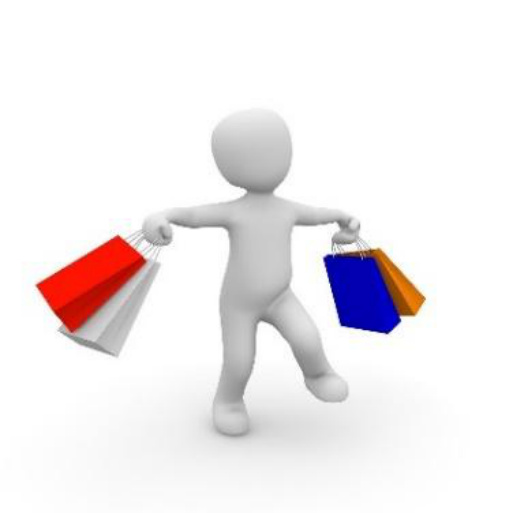
\includegraphics[height=1.1cm,keepaspectratio]{images/img_p45_1_222.jpeg}
\end{center}
\end{column}
\end{columns}
\end{frame}

% Slide 38: Classification Definition
\begin{frame}{مسئله دسته‌بندی}{\lr{Classification}}
\begin{columns}[T,onlytextwidth]
\begin{column}{0.75\textwidth}
\begin{itemize}\setlength{\itemsep}{5pt}
  \item \textbf{تعریف هدف:}
  \begin{itemize}\setlength{\itemsep}{2pt}
    \item تخصیص دقیق رکوردهای جدید و دیده‌نشده به یکی از کلاس‌های از پیش تعیین‌شده با بالاترین دقت ممکن.
  \end{itemize}
  \item \textbf{رویکرد یادگیری:}
  \begin{itemize}\setlength{\itemsep}{3pt}
    \item با داشتن مجموعه‌ای از داده‌های آموزشی \lr{(Training Set)}:
    \begin{itemize}\setlength{\itemsep}{2pt}
      \item هر رکورد شامل مجموعه‌ای از ویژگی‌ها \lr{(Attributes)} است.
      \item یکی از ویژگی‌ها، برچسب کلاس هدف \lr{(Class Label)} است.
    \end{itemize}
    \item برازش مدلی که برچسب کلاس را به عنوان تابعی از سایر ویژگی‌ها پیش‌بینی کند:
    \begin{center}
    \begin{latin}
    $y = f(\mathbf{x}) = f(x_1, x_2, \dots, x_d)$
    \end{latin}
    \end{center}
  \end{itemize}
\end{itemize}
\end{column}%
\begin{column}{0.22\textwidth}
\begin{center}
  \vspace{0.3cm}
  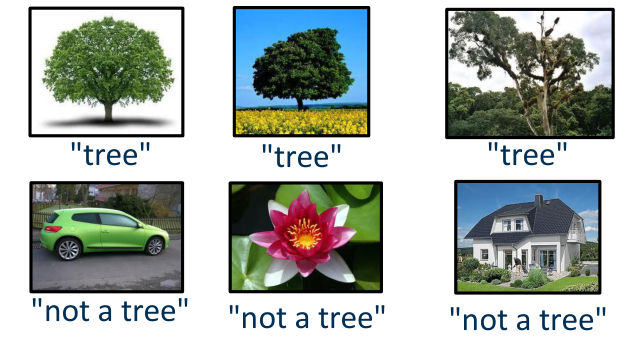
\includegraphics[width=\linewidth,keepaspectratio]{images/thumb_trees_classification.png}
\end{center}
\end{column}
\end{columns}
\end{frame}

% Slide 39: Classification Visual Example
\begin{frame}{مثال شهودی مسئله دسته‌بندی}
\framesubtitle{تشخیص درخت (\lr{Tree}) از غیر درخت (\lr{Not a Tree})}
\begin{center}
  {\small\color{mannheimblue}\textbf{نمونه‌های مثبت (کلاس درخت -- \lr{``tree''})}}\\[0.1cm]
  \begin{LTR}
  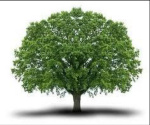
\includegraphics[width=0.3\textwidth,height=2cm,keepaspectratio]{images/img_p37_2_192.jpeg}\hspace{0.2cm}
  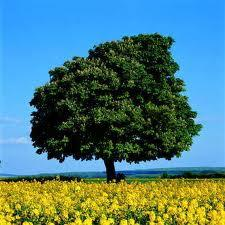
\includegraphics[width=0.3\textwidth,height=2cm,keepaspectratio]{images/img_p37_3_193.jpeg}\hspace{0.2cm}
  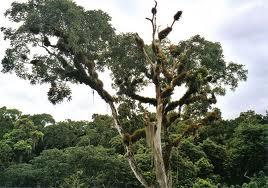
\includegraphics[width=0.3\textwidth,height=2cm,keepaspectratio]{images/img_p37_4_194.jpeg}
  \end{LTR}
  \par\vspace{0.25cm}
  {\small\color{mannheimgold}\textbf{نمونه‌های منفی (کلاس غیر درخت -- \lr{``not a tree''})}}\\[0.1cm]
  \begin{LTR}
  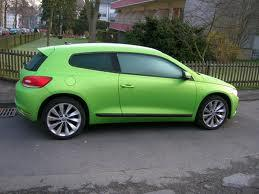
\includegraphics[width=0.3\textwidth,height=2cm,keepaspectratio]{images/img_p37_5_195.jpeg}\hspace{0.2cm}
  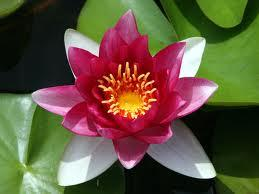
\includegraphics[width=0.3\textwidth,height=2cm,keepaspectratio]{images/img_p37_6_196.jpeg}\hspace{0.2cm}
  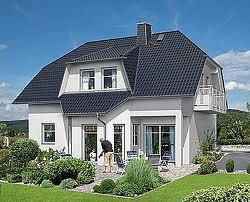
\includegraphics[width=0.3\textwidth,height=2cm,keepaspectratio]{images/img_p37_7_197.jpeg}
  \end{LTR}
\end{center}
\end{frame}

% Slide 40: Classification Workflow
\begin{frame}{جریان کاری و مراحل مدل‌سازی دسته‌بندی}
\begin{center}
  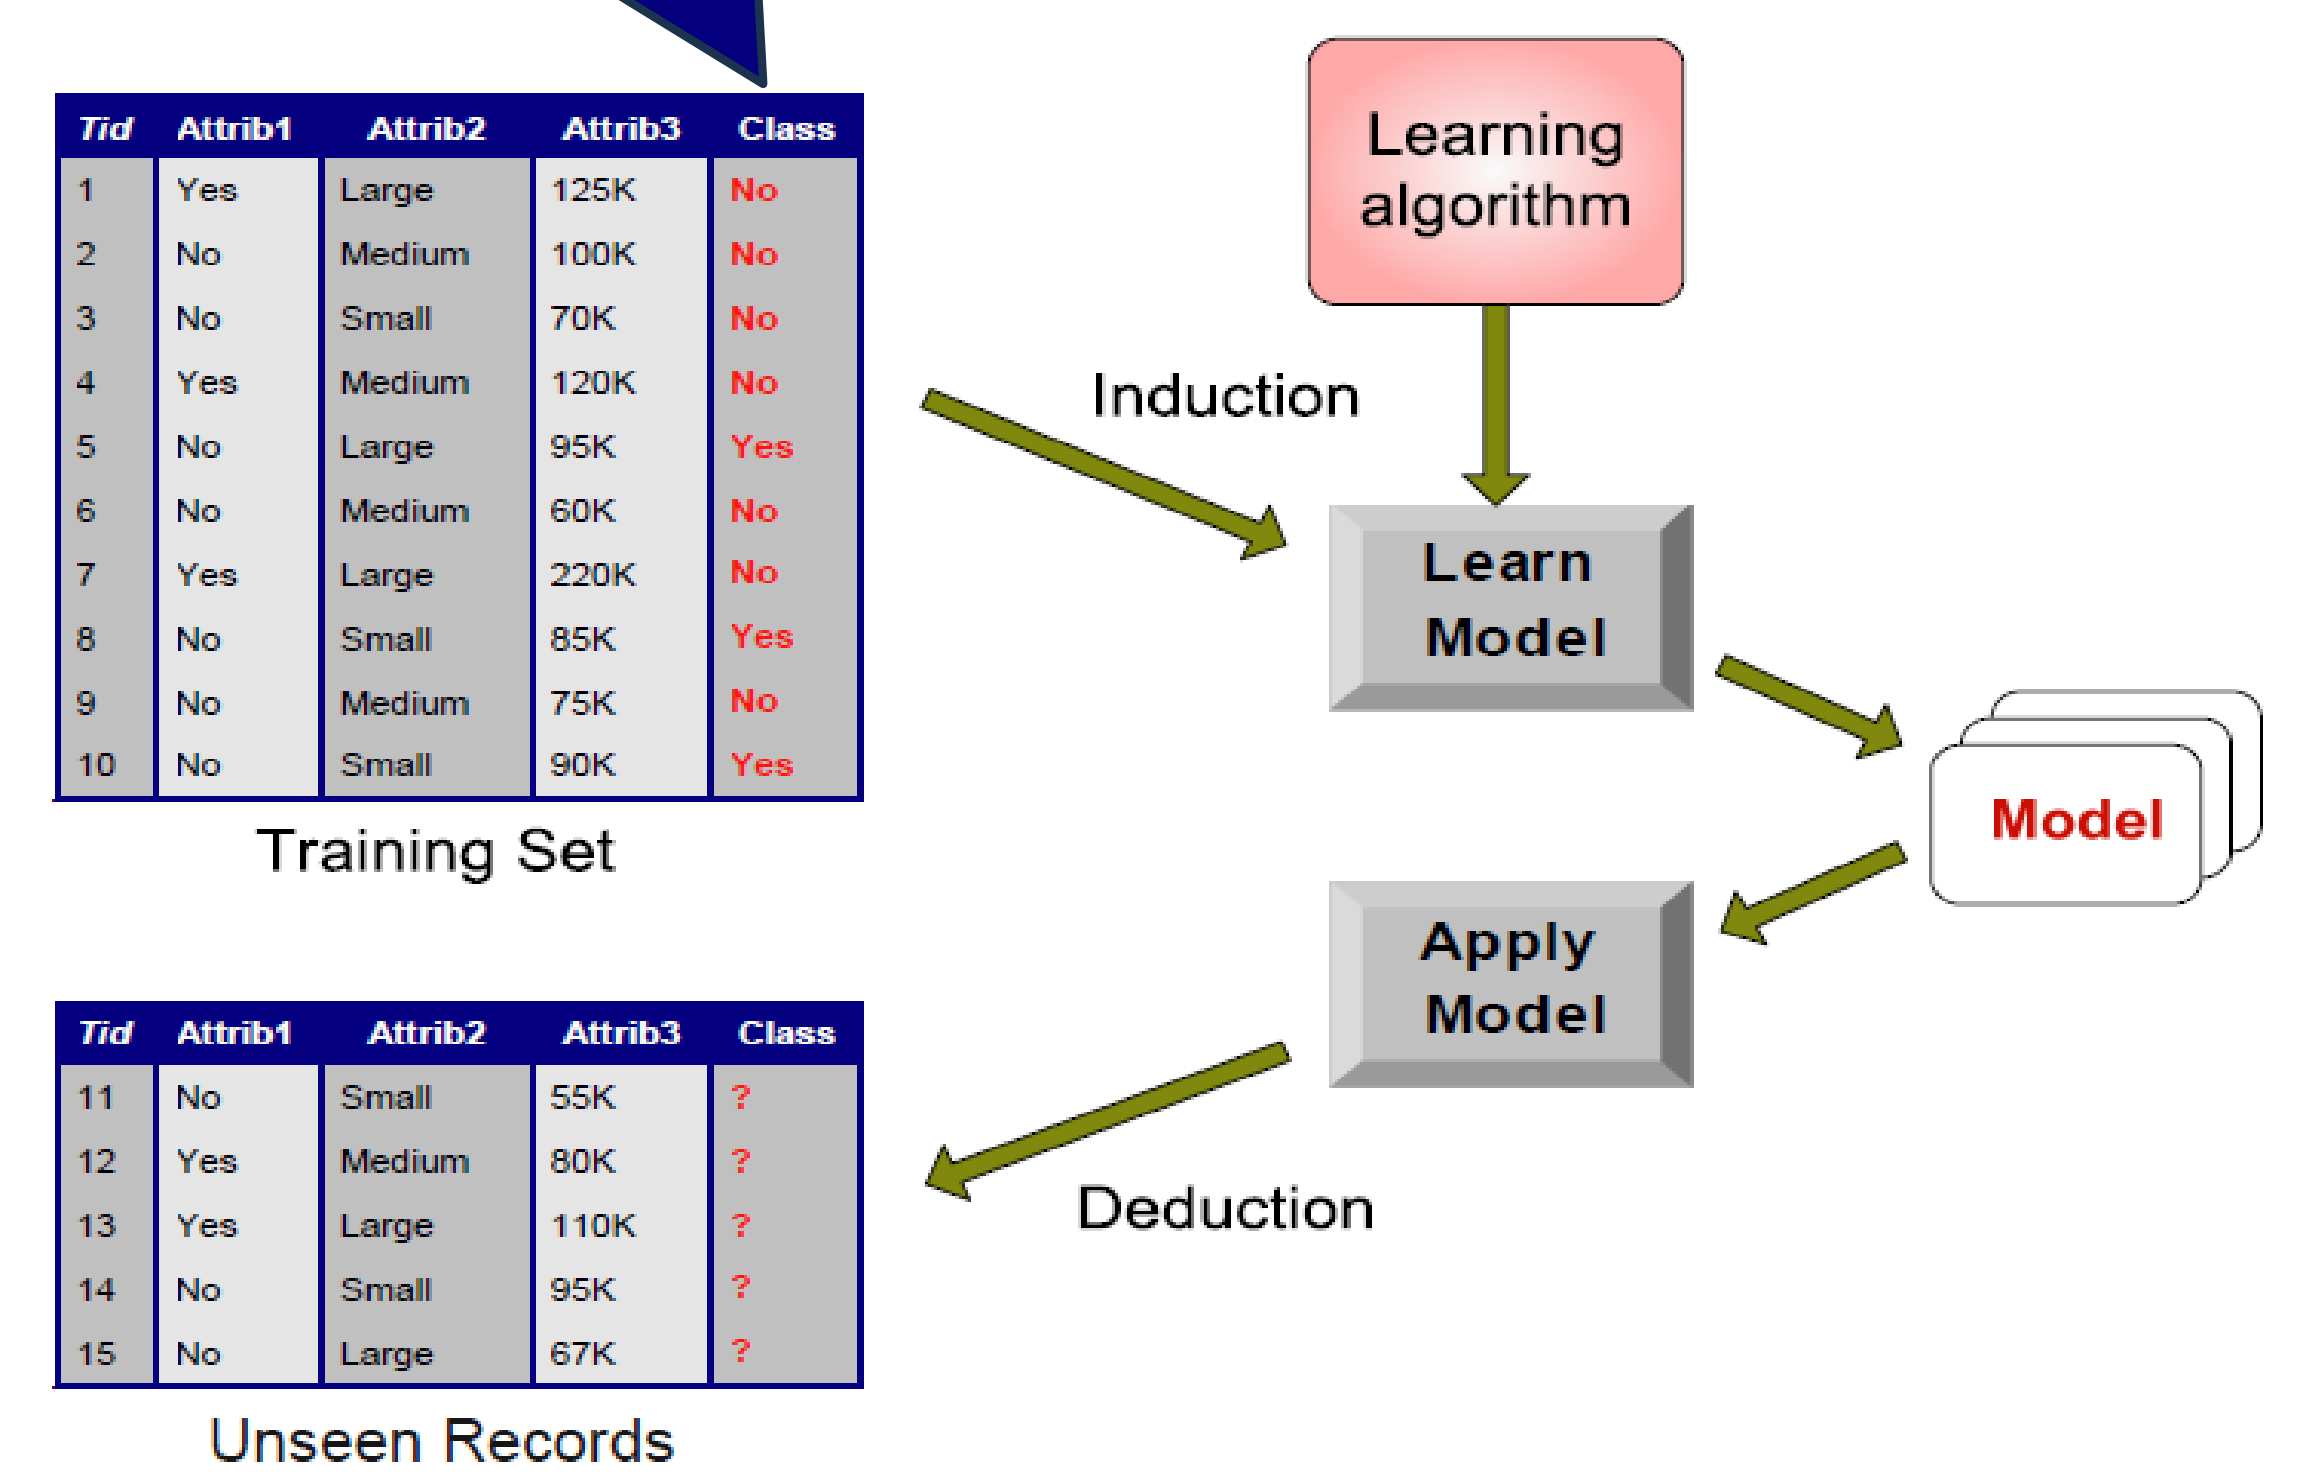
\includegraphics[width=0.88\textwidth,height=4.3cm,keepaspectratio]{images/img_p40_1_205.png}\\[0.1cm]
  {\fontsize{7}{9}\selectfont\color{subgray}آموزش مدل روی داده‌های برچسب‌دار و ارزیابی روی داده‌های آزمون برای پیش‌بینی برچسب ناشناخته}
\end{center}
\end{frame}

% Slide 41: Classification Applications
\begin{frame}{کاربردهای عملی دسته‌بندی}
\begin{columns}[T,onlytextwidth]
\begin{column}{0.65\textwidth}
\begin{itemize}
  \item \textbf{ارزیابی ریسک اعتباری بانکی} (\lr{Credit Risk})
  \begin{itemize}
    \item \textbf{ویژگی‌ها:} سن، سطح درآمد، بدهی‌های جاری، سابقه مالی
    \item \textbf{کلاس:} اعطای وام توسط بانک؟ (بله / خیر)
  \end{itemize}
  \vspace{0.15cm}
  \item \textbf{تشخیص ایمیل‌های هرزنامه} (\lr{SPAM Detection})
  \begin{itemize}
    \item \textbf{ویژگی‌ها:} کلمات متن، فیلدهای هدر ایمیل، فرستنده
    \item \textbf{کلاس:} ایمیل عادی (\lr{Ham}) یا هرزنامه (\lr{Spam})
  \end{itemize}
  \vspace{0.15cm}
  \item \textbf{کشف تقلب در اظهارنامه‌های مالیاتی} (\lr{Tax Fraud})
  \begin{itemize}
    \item \textbf{ویژگی‌ها:} ارقام و نسبت‌های مالیاتی اظهارشده
    \item \textbf{کلاس:} سوءاستفاده مالیاتی؟ (نیازمند بازرسی / عادی)
  \end{itemize}
\end{itemize}
\end{column}
\begin{column}{0.32\textwidth}
\begin{center}
  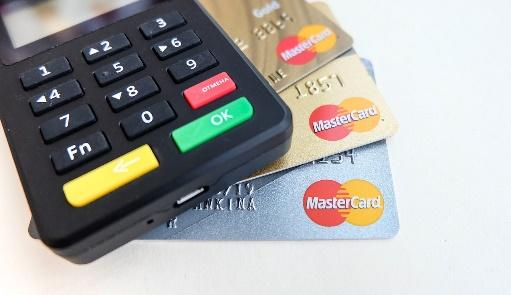
\includegraphics[width=0.85\textwidth,height=1.4cm,keepaspectratio]{images/img_p41_3_210.jpeg}\\[0.1cm]
  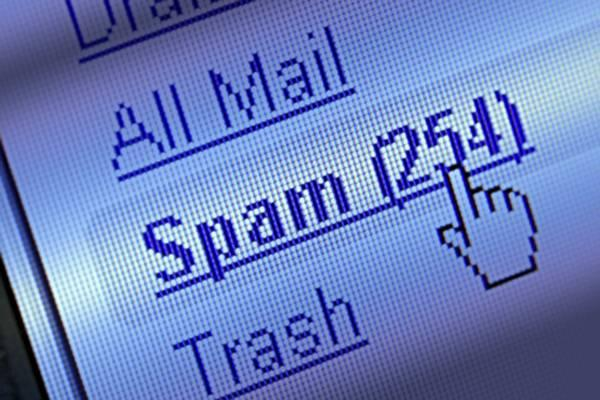
\includegraphics[width=0.85\textwidth,height=1.4cm,keepaspectratio]{images/img_p41_1_208.jpeg}\\[0.1cm]
  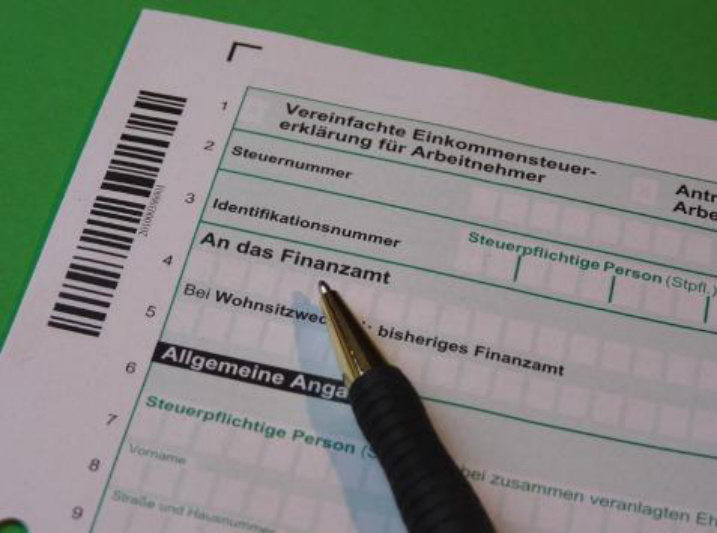
\includegraphics[width=0.85\textwidth,height=1.4cm,keepaspectratio]{images/img_p41_2_209.jpeg}
\end{center}
\end{column}
\end{columns}
\end{frame}

% Slide 42: Regression
\begin{frame}{مسئله رگرسیون (\lr{Regression})}
\begin{columns}[c,onlytextwidth]
\begin{column}{0.65\textwidth}
\begin{itemize}
  \item \textbf{پیش‌بینی متغیرهای عددی و پیوسته:}
  \begin{itemize}
    \item تخمین مقدار یک ویژگی پیوسته بر پایه سایر متغیرها
    \item برازش مدل‌های رگرسیون خطی یا غیرخطی
  \end{itemize}
  \vspace{0.1cm}
  \item \textbf{نمونه‌های کاربردی:}
  \begin{itemize}
    \item پیش‌بینی قیمت مسکن، خودرو یا ارزش دارایی‌ها
    \item پیش‌بینی حجم فروش بر پایه بودجه تبلیغاتی
    \item تخمین مصرف سوخت خودرو (\lr{MPG}) بر پایه وزن و توان
  \end{itemize}
\end{itemize}
\end{column}
\begin{column}{0.32\textwidth}
\begin{center}
  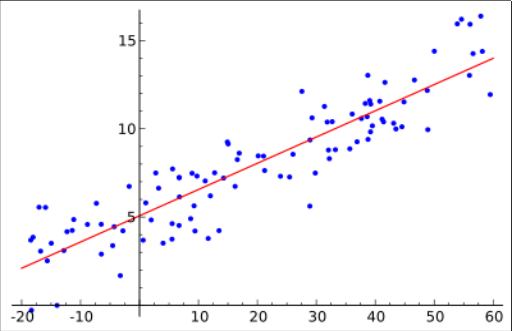
\includegraphics[width=\textwidth,height=1.7cm,keepaspectratio]{images/img_p37_8_198.png}\\[0.15cm]
  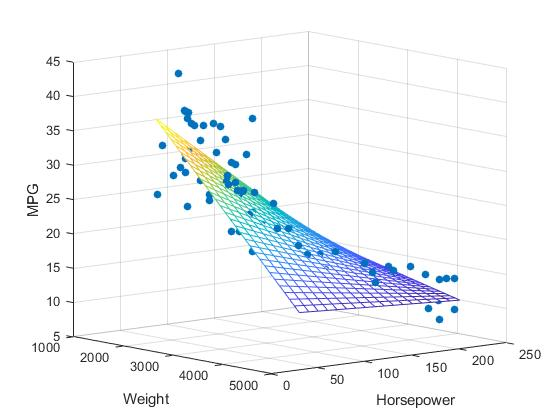
\includegraphics[width=\textwidth,height=1.7cm,keepaspectratio]{images/img_p42_2_213.jpeg}
\end{center}
\end{column}
\end{columns}
\vspace{0.2cm}
\begin{itemize}
  \item \textbf{تفاوت بنیادین با دسته‌بندی:} رگرسیون متغیر پیوسته عددی را تخمین می‌زند، در حالی که دسته‌بندی برای برچسب‌های کیفی و گسسته به کار می‌رود.
\end{itemize}
\end{frame}

% Slide 43: Cluster Analysis
\begin{frame}{تحلیل خوشه‌بندی (\lr{Cluster Analysis})}
\begin{columns}[c,onlytextwidth]
\begin{column}{0.56\textwidth}
\begin{itemize}
  \item \textbf{تعریف هدف:}
  \begin{itemize}
    \item گروه‌بندی داده‌ها بر مبنای شباهت ذاتی:
    \item شباهت بیشینه میان اعضای درون هر خوشه
    \item شباهت کمینه میان اعضای خوشه‌های مجزا
  \end{itemize}
  \vspace{0.15cm}
  \item \textbf{معیارهای شباهت} (\lr{Similarity Measures})
  \begin{itemize}
    \item فاصله اقلیدسی برای متغیرهای پیوسته
    \item شباهت کسینوسی یا جاکارد
  \end{itemize}
  \vspace{0.15cm}
  \item \textbf{اهداف بهینه‌سازی:}
  \begin{itemize}
    \item کمینه‌سازی فواصل درون‌خوشه‌ای (\lr{Intra-cluster})
    \item بیشینه‌سازی فواصل بین‌خوشه‌ای (\lr{Inter-cluster})
  \end{itemize}
\end{itemize}
\end{column}
\begin{column}{0.42\textwidth}
\begin{center}
  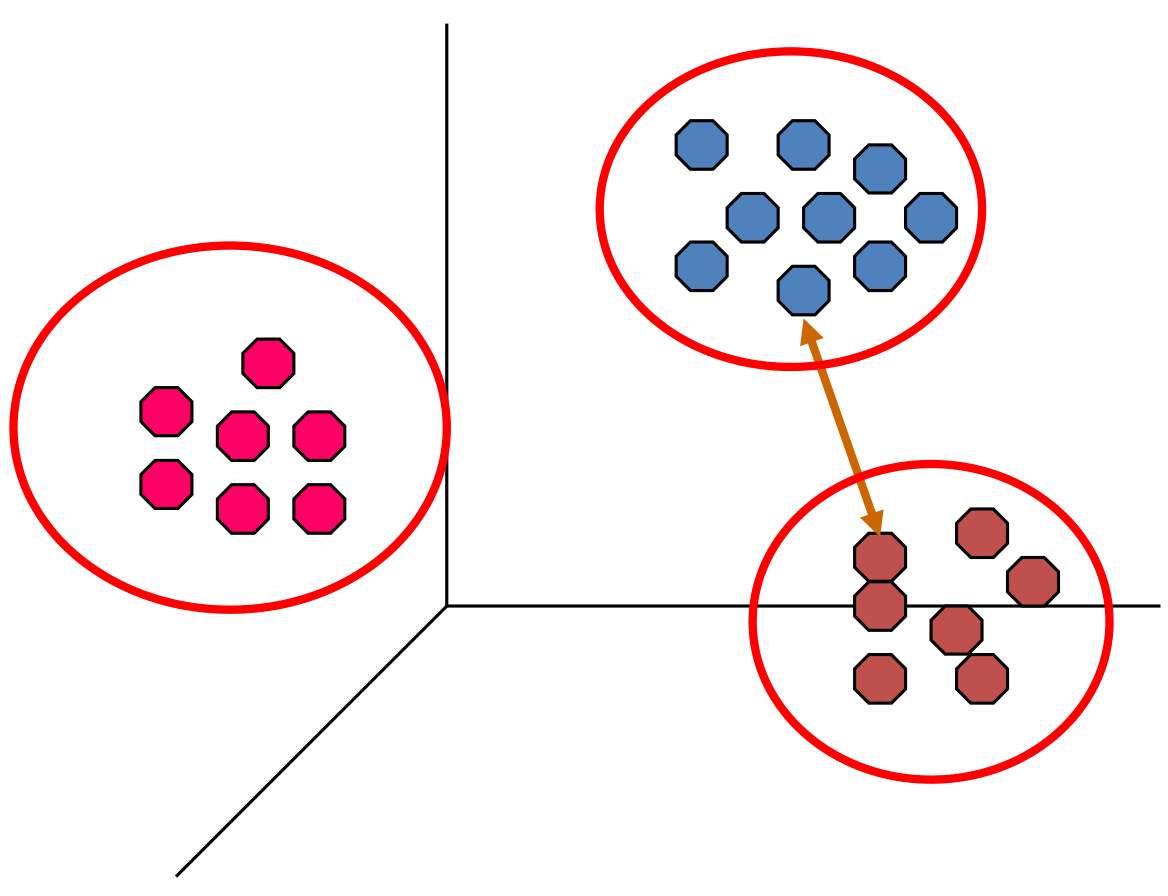
\includegraphics[width=\textwidth,height=3.8cm,keepaspectratio]{images/diagram_p43_cluster_drawing.png}
\end{center}
\end{column}
\end{columns}
\end{frame}

% Slide 44: Cluster Analysis Applications
\begin{frame}{کاربردهای عملی خوشه‌بندی}
\begin{columns}[c,onlytextwidth]
\begin{column}{0.62\textwidth}
\begin{itemize}
  \item \textbf{کاربرد اول -- بخش‌بندی بازار} (\lr{Market Segmentation})
  \begin{itemize}
    \item شناسایی خوشه‌های مشتریان با رفتار مشابه
    \item طراحی کمپین‌های تبلیغاتی متناسب برای هر بخش
  \end{itemize}
  \vspace{0.25cm}
  \item \textbf{کاربرد دوم -- خوشه‌بندی اسناد متنی} (\lr{Document Clustering})
  \begin{itemize}
    \item گروه‌بندی خودکار اخبار بر مبنای واژگان
    \item نمونه: تجمیع اخبار در اخبار گوگل (\lr{Google News})
  \end{itemize}
\end{itemize}
\end{column}
\begin{column}{0.35\textwidth}
\begin{center}
  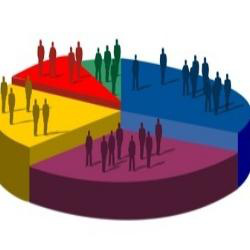
\includegraphics[width=0.85\textwidth,height=2cm,keepaspectratio]{images/img_p44_1_218.png}\\[0.2cm]
  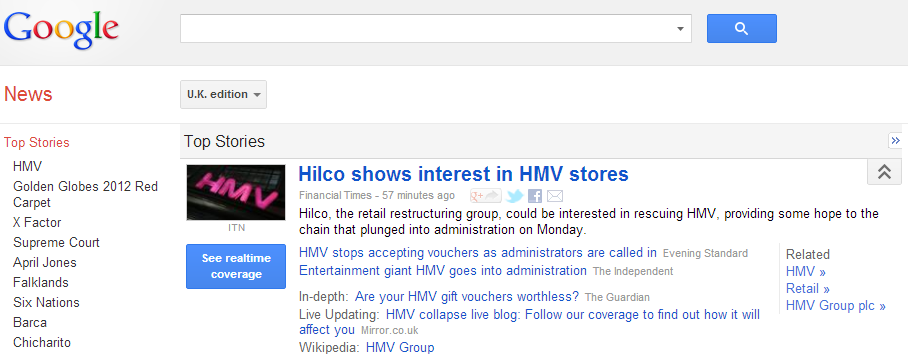
\includegraphics[width=\textwidth,height=2cm,keepaspectratio]{images/img_p44_2_219.jpeg}
\end{center}
\end{column}
\end{columns}
\end{frame}

% Slide 45: Association Analysis
\begin{frame}{تحلیل وابستگی (\lr{Association Analysis})}
\begin{itemize}
  \item \textbf{صورت مسئله:} تراکنش‌های سبد خرید شامل مجموعه‌ای از اقلام
  \item \textbf{هدف:} کشف مجموعه‌های مکرر و استخراج قوانین وابستگی جهت پیش‌بینی
\end{itemize}
\vspace{0.1cm}
\begin{columns}[c,onlytextwidth]
\begin{column}{0.48\textwidth}
\begin{center}
{\scriptsize
\begin{tabular}{cl}
\toprule
\textbf{شناسه (\lr{TID})} & \textbf{اقلام خریداری‌شده (\lr{Items})} \\
\midrule
1 & \lr{Bread, Coke, Milk} \\
2 & \lr{Beer, Bread} \\
3 & \lr{Beer, Coke, Diaper, Milk} \\
4 & \lr{Beer, Bread, Diaper, Milk} \\
5 & \lr{Coke, Diaper, Milk} \\
\bottomrule
\end{tabular}
}
\end{center}
\end{column}
\begin{column}{0.48\textwidth}
\begin{block}{\footnotesize مجموعه‌های مکرر (\lr{Frequent Itemsets})}
  \centering\vspace{0.05cm}
  {\small\lr{\{Diaper, Milk, Beer\}}}\\
  {\small\lr{\{Milk, Coke\}}}
\end{block}
\vspace{0.15cm}
\begin{block}{\footnotesize قوانین وابستگی (\lr{Association Rules})}
  \centering\vspace{0.05cm}
  {\small\lr{\{Diaper, Milk\} $\rightarrow$ \{Beer\}}}\\
  {\small\lr{\{Milk\} $\rightarrow$ \{Coke\}}}
\end{block}
\end{column}
\end{columns}
\end{frame}

% Slide 46: Association Analysis Applications
\begin{frame}{کاربردهای عملی قواعد وابستگی}
\begin{columns}[c,onlytextwidth]
\begin{column}{0.65\textwidth}
\begin{itemize}
  \item \textbf{مدیریت چیدمان قفسه‌ها} (\lr{Shelf Management})
  \begin{itemize}
    \item شناسایی کالاهایی که با هم خریده می‌شوند
    \item پردازش داده‌های بارکدخوان صندوق فروشگاه
  \end{itemize}
  \vspace{0.25cm}
  \item \textbf{ترفیع فروش و پیشنهادهای مکمل} (\lr{Sales Promotion})
  \begin{itemize}
    \item طراحی تخفیف‌های ترکیبی روی اقلام مرتبط
    \item پیشنهاد خودکار اقلام مکمل در فروشگاه اینترنتی
  \end{itemize}
\end{itemize}
\end{column}
\begin{column}{0.32\textwidth}
\begin{center}
  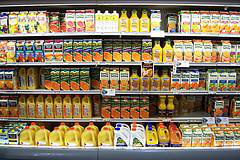
\includegraphics[width=\textwidth,height=1.8cm,keepaspectratio]{images/img_p46_2_244.jpeg}\\[0.2cm]
  
\includegraphics[width=0.7\textwidth,height=0.7cm,keepaspectratio]{images/img_p46_1_243.jpeg}\\[0.1cm]
  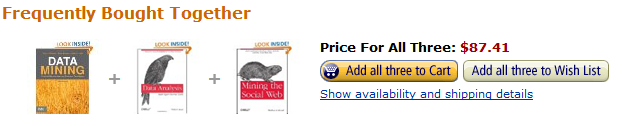
\includegraphics[width=\textwidth,height=1.2cm,keepaspectratio]{images/img_p46_3_245.png}
\end{center}
\end{column}
\end{columns}
\end{frame}

% Slide 47: Which Methods are Used in Practice?
\begin{frame}{کدام روش‌ها در عمل بیشترین کاربرد را دارند؟}
\begin{itemize}
  \item \textbf{نظرسنجی معتبر پایگاه \lr{KDnuggets} از فعالان صنعت داده:}
\end{itemize}
\begin{center}
  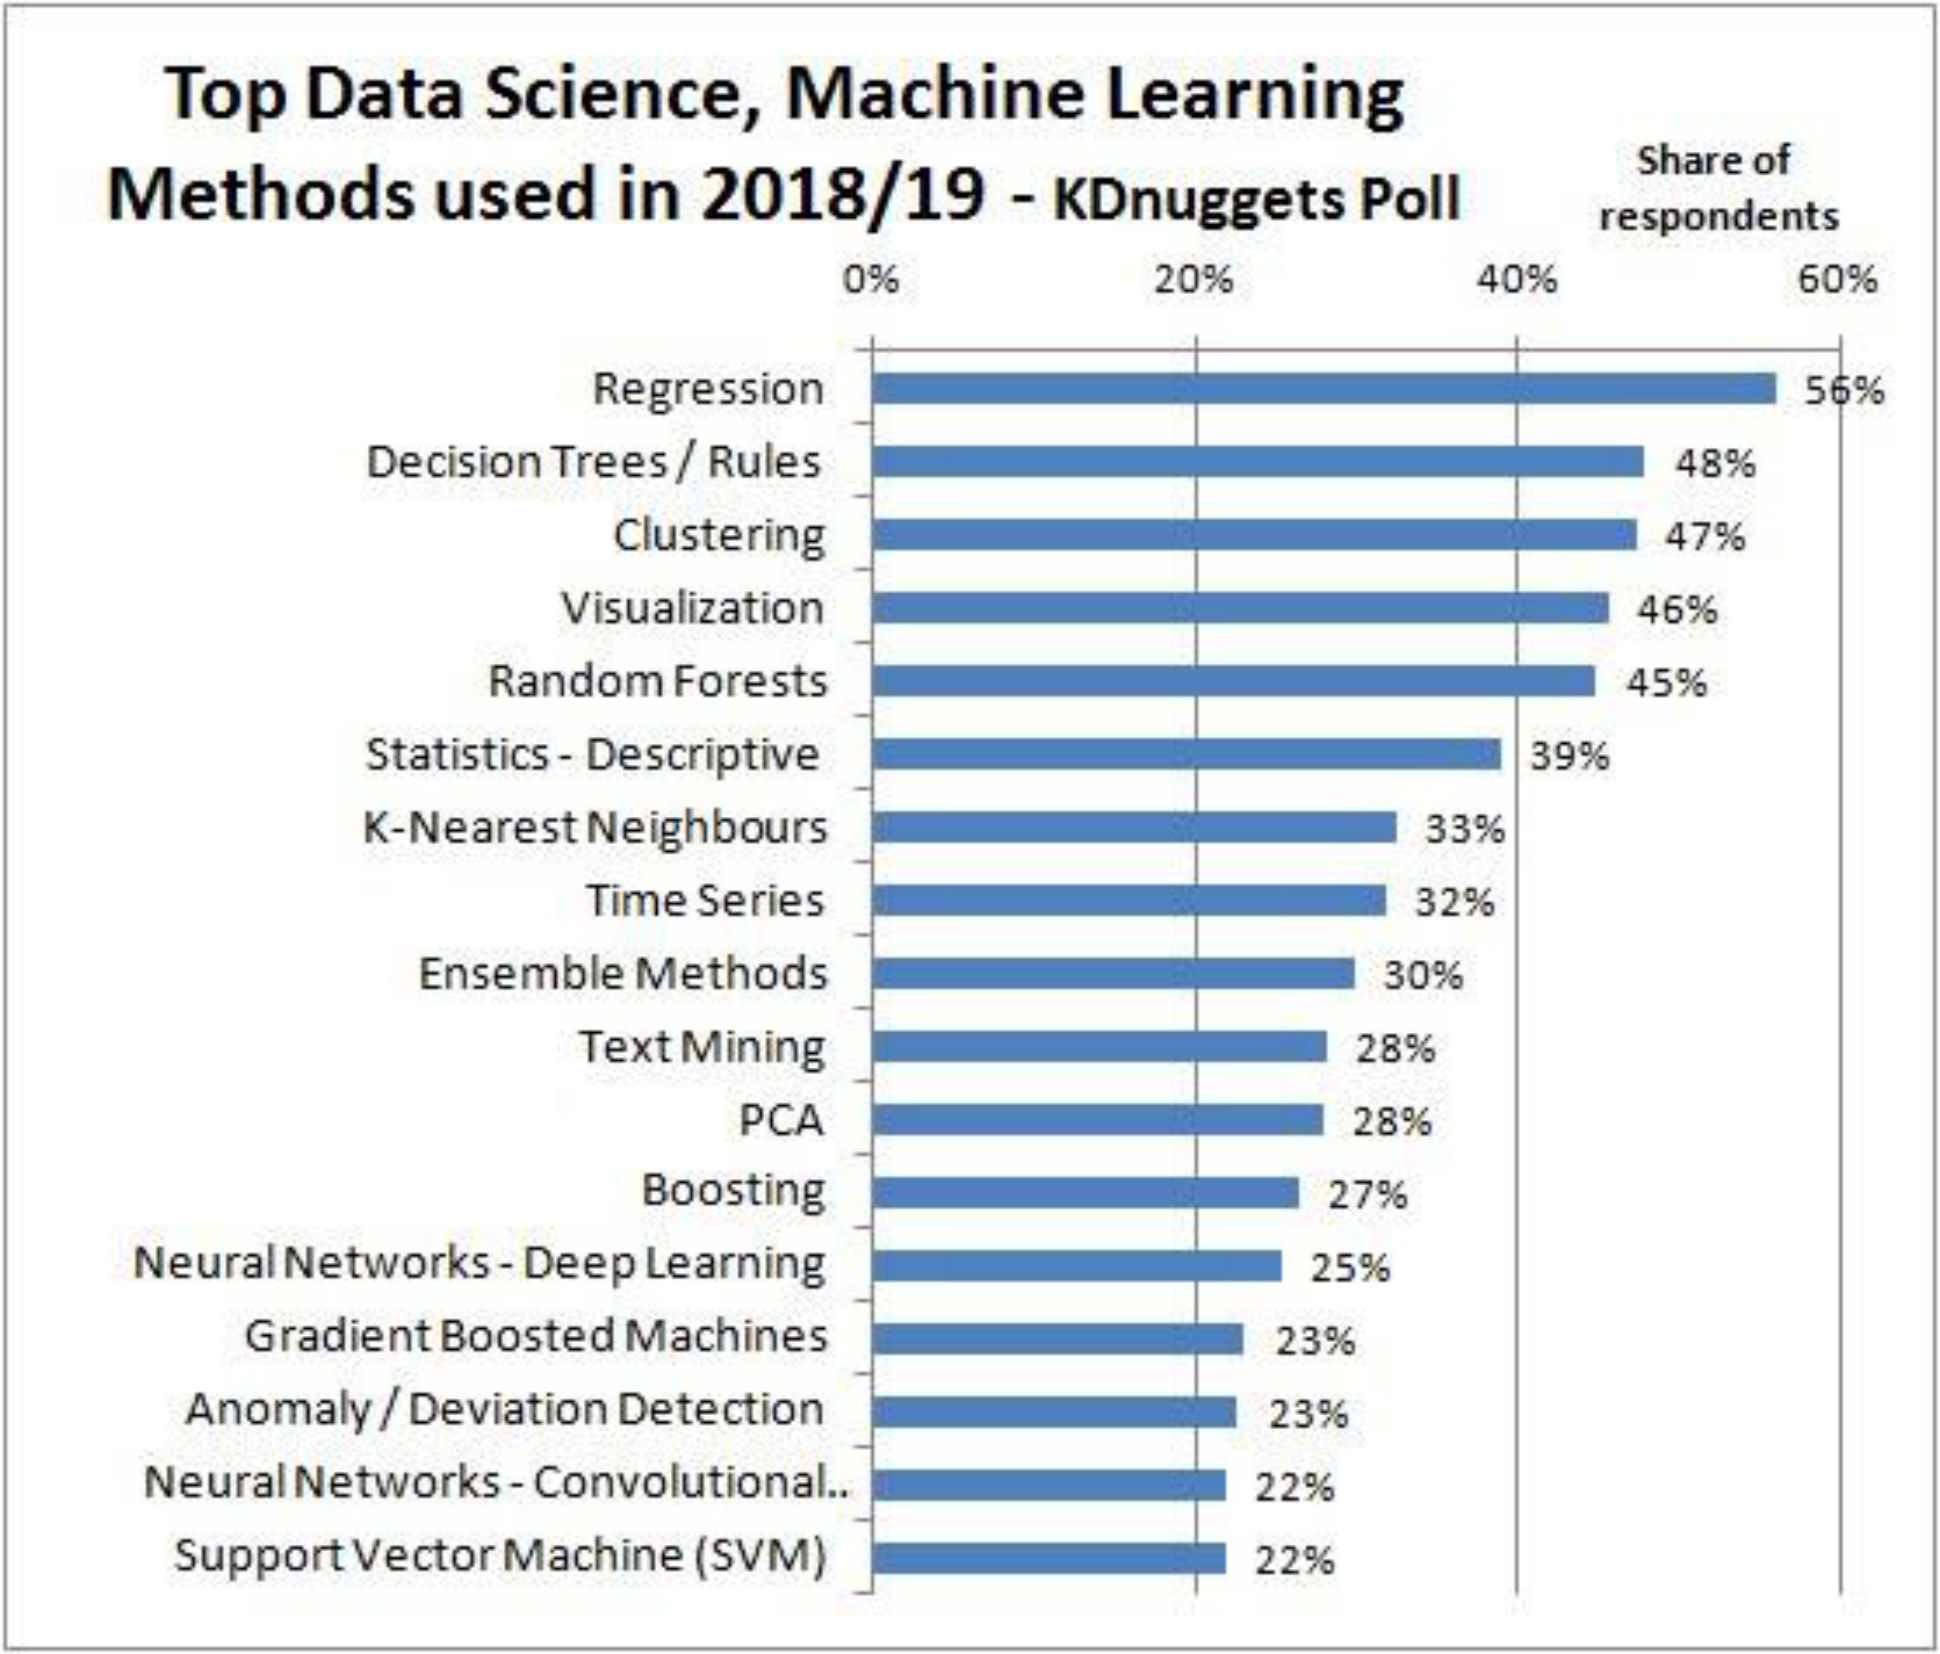
\includegraphics[width=0.72\textwidth,height=4.3cm,keepaspectratio]{images/img_p47_1_248.jpeg}\\[0.1cm]
  {\fontsize{6.8}{8}\selectfont\color{subgray}رگرسیون، درخت‌های تصمیم و خوشه‌بندی همچنان در صدر پرکاربردترین متدهای صنعتی قرار دارند}
\end{center}
\end{frame}
